\chapter{Fault Modeling and the Safety Annex}
\ref{chap:faultModeling}
\danielle{This chapter covers modeling techniques/needs, the safety annex, and its capabilities.}

\section{Component Fault Modeling}
The usage of the terms error, failure, and fault are defined in ARP4754A and are described here for ease of understanding~\cite{SAE:ARP4754A}. An \textit{error} is a mistake made in implementation, design, or requirements. A \textit{fault} is the manifestation of an error and a \textit{failure} is an event that occurs when the delivered service of a system deviates from correct behavior. If a fault is activated under the right circumstances, that fault can lead to a failure. The terminology used in EMV2 differs slightly for an error: an error is a corrupted state caused by a fault. The error propagates through a system and can  manifest as a failure. In this report, we use the ARP4754A terminology with the added definition of \textit{error propagation} as used in EMV2. An error is a mistake made in design or code and an error propagation is the propagation of the corrupted state caused by an active fault. 

The Safety Annex is used to add possible faulty behaviors to a component model. Within the AADL component instance model, an annex is added which contain the fault definitions for the given component. The flexibility of the fault definitions allows the user to define numerous types of fault \textit{nodes} by utilizing the AGREE node syntax. A library of common fault nodes has been written and is available in the project GitHub repository~\cite{SAGithub}. Examples of such faults include valves being stuck open or closed, output of a software component being nondeterministic, or power being cut off.  When the fault analysis requires fault definitions that are more complex, these nodes can easily be written and used in the model. 

When a fault is activated by its specified triggering conditions, it modifies the output of the component. This faulty behavior may violate the contracts of other components in the system, including assumptions of downstream components. The impact of a fault is computed by the AGREE model checker when the safety analysis is run on the fault model. 

The majority of faults that are connected to outputs of components are known as \textit{symmetric}. That is, whatever components receive this faulty output will receive the same faulty output value. Thus, this output is seen symmetrically. An alternative fault type is \textit{asymmetric}. This pertains to a component with a 1-n output: one output which is sent to many receiving components. This fault can present itself differently to the receiving components. For instance, in a boolean setting, one component might see a true value and the rest may see false. This is also possible to model using the keyword \textit{asymmetric}. For more information on fault definitions and modeling possibilities, we refer readers to the Safety Annex Users Guide\cite{SAGithub}.

As an illustration of fault modeling using the Safety Annex, we look at one of the components important to the inadvertent braking property: the brake pedal. When the mechanical pedal is pressed, a sensor reads this information and passes an electronic signal to the BSCU which then commands hydraulic pressure to the wheels. 

%Figure~\ref{fig:sensor} 
Figure~\ref{fig:sensor} shows the AADL pedal sensor component with a contract for its nominal behavior. The sensor has only one input, the mechanical pedal position, and one output, the electrical pedal position. 
A property that governs the behavior of the component is that the mechanical position should always equal the electronic position. (The expression \textit{true $\rightarrow$ property} in AGREE is true in the initial state and then afterwards it is only true if property holds.)

\begin{figure}[h!]
	\hspace*{-2cm}
	%\vspace{-0.55in} 
	\begin{center}
		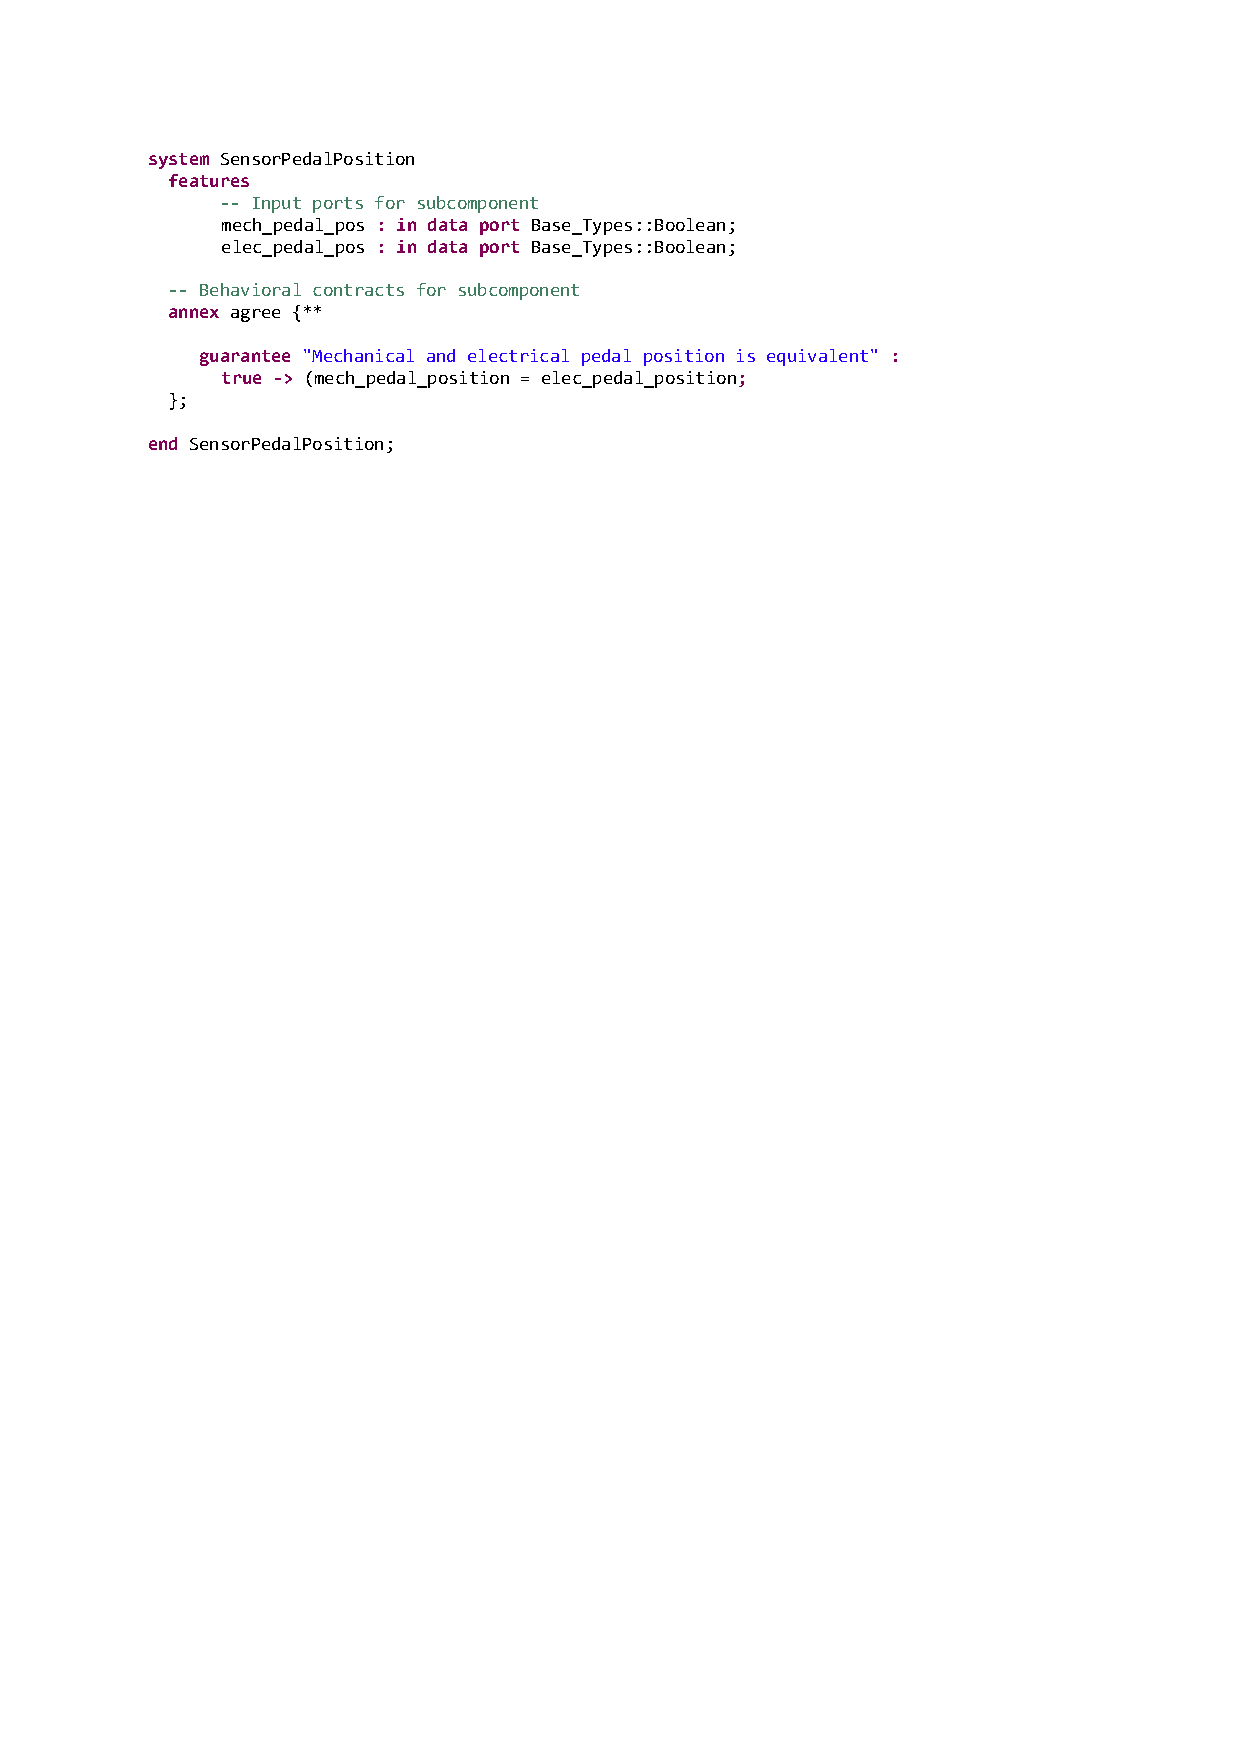
\includegraphics[trim=0 640 -10 70,clip,width=1.5\dimexpr\textwidth-2cm\relax]{images/system_sensor.pdf}
		\vspace{-0.3in}
		\caption{An AADL System Type: The Pedal Sensor}
		\label{fig:sensor}
	\end{center}
	\vspace{-0.2in}
\end{figure}

One possible failure for this sensor is inversion of its output value. This fault can be triggered with probability $5.0\times 10^{-6}$ as described in AIR6110 (in reality, the component failure probability is 
collected from hardware specification sheets).  
The Safety Annex definition for this fault is shown in Figure~\ref{fig:sensorFault}. Fault behavior is defined through the use of a fault node called \textit{inverted\_fail}.  When the fault is triggered, the nominal output of the component (\textit{elec\_pedal\_position}) is replaced with its failure value (\textit{val\_out}). 

\begin{figure}[h!]
	\hspace*{-2cm}
	%\vspace{-0.5in} 
	\begin{center}
		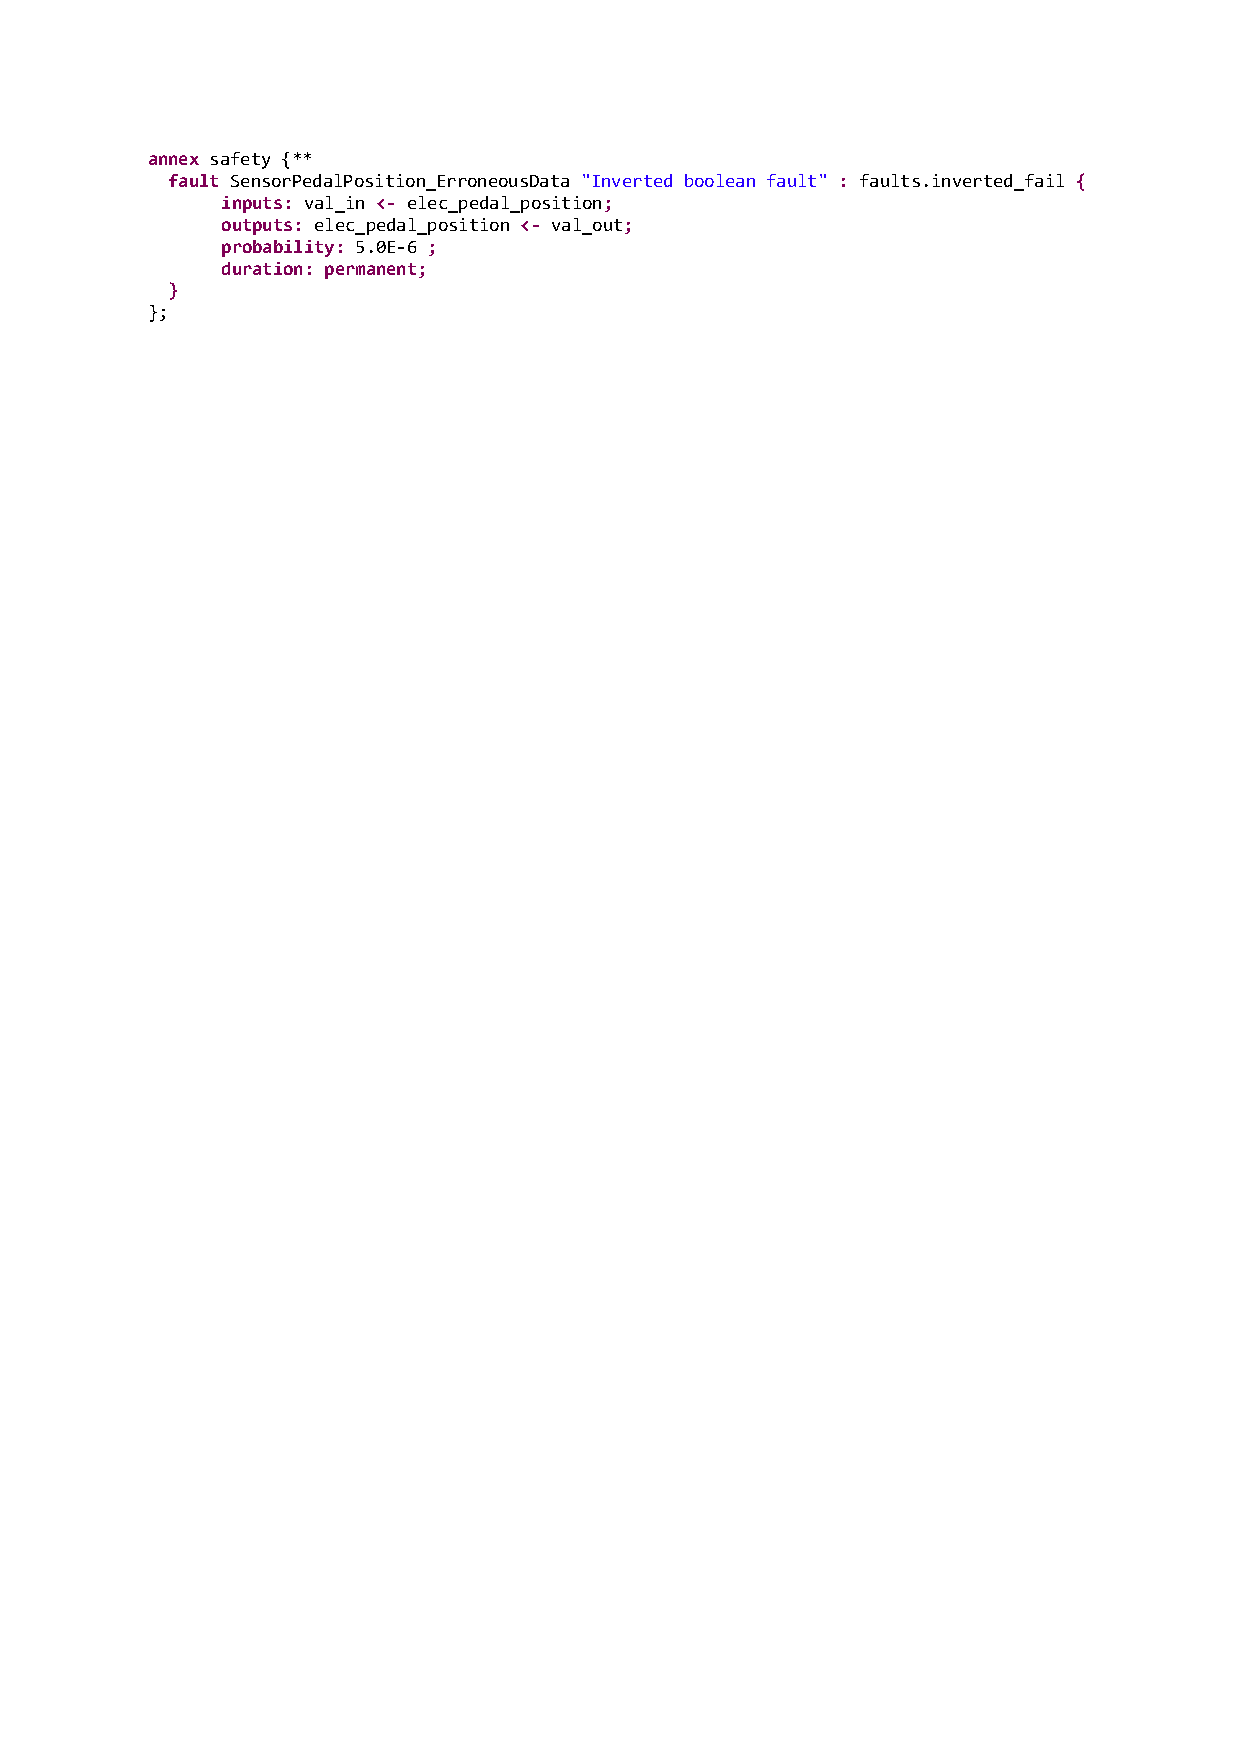
\includegraphics[trim=0 680 -10 70,clip,width=1.5\dimexpr\textwidth-2cm\relax]{images/safetyannex_sensorfault.pdf}
		\vspace{-0.2in}
		\caption{The Safety Annex for the Pedal Sensor}
		\label{fig:sensorFault}
	\end{center}
	\vspace{-0.2in}
\end{figure}

The WBS fault model expressed in the Safety Annex contains a total of 33 different fault types and 141 fault instances. The large number of fault instances is due to the redundancy in the system design and its replication to control 8 wheels.

\section{Error Propagation}

\subsection{Implicit Propagation}
In the Safety Annex approach, faults are captured as faulty behaviors that augment the system behavioral model in AGREE contracts. No explicit %fault
error propagation is necessary since the faulty behavior itself propagates through the system just as in the nominal system model. The effects of any triggered fault are manifested through analysis of the AGREE contracts. 

On the contrary, in the AADL Error Model Annex, Version 2 (EMV2)~\cite{EMV2} approach, all errors must be explicitly propagated through each component (by applying fault types on each of the output ports) in order for a component to have an impact on the rest of the system. To illustrate the key differences between implicit %failure
error propagation provided in the Safety Annex and the explicit %failure 
error propagation provided in EMV2, we use a simplified behavioral flow from the WBS example using code fragments from EMV2, AGREE, and the Safety Annex. 

\begin{figure}[t]
	\hspace*{-2cm}
	\vspace{-0.19in}
	\centering
	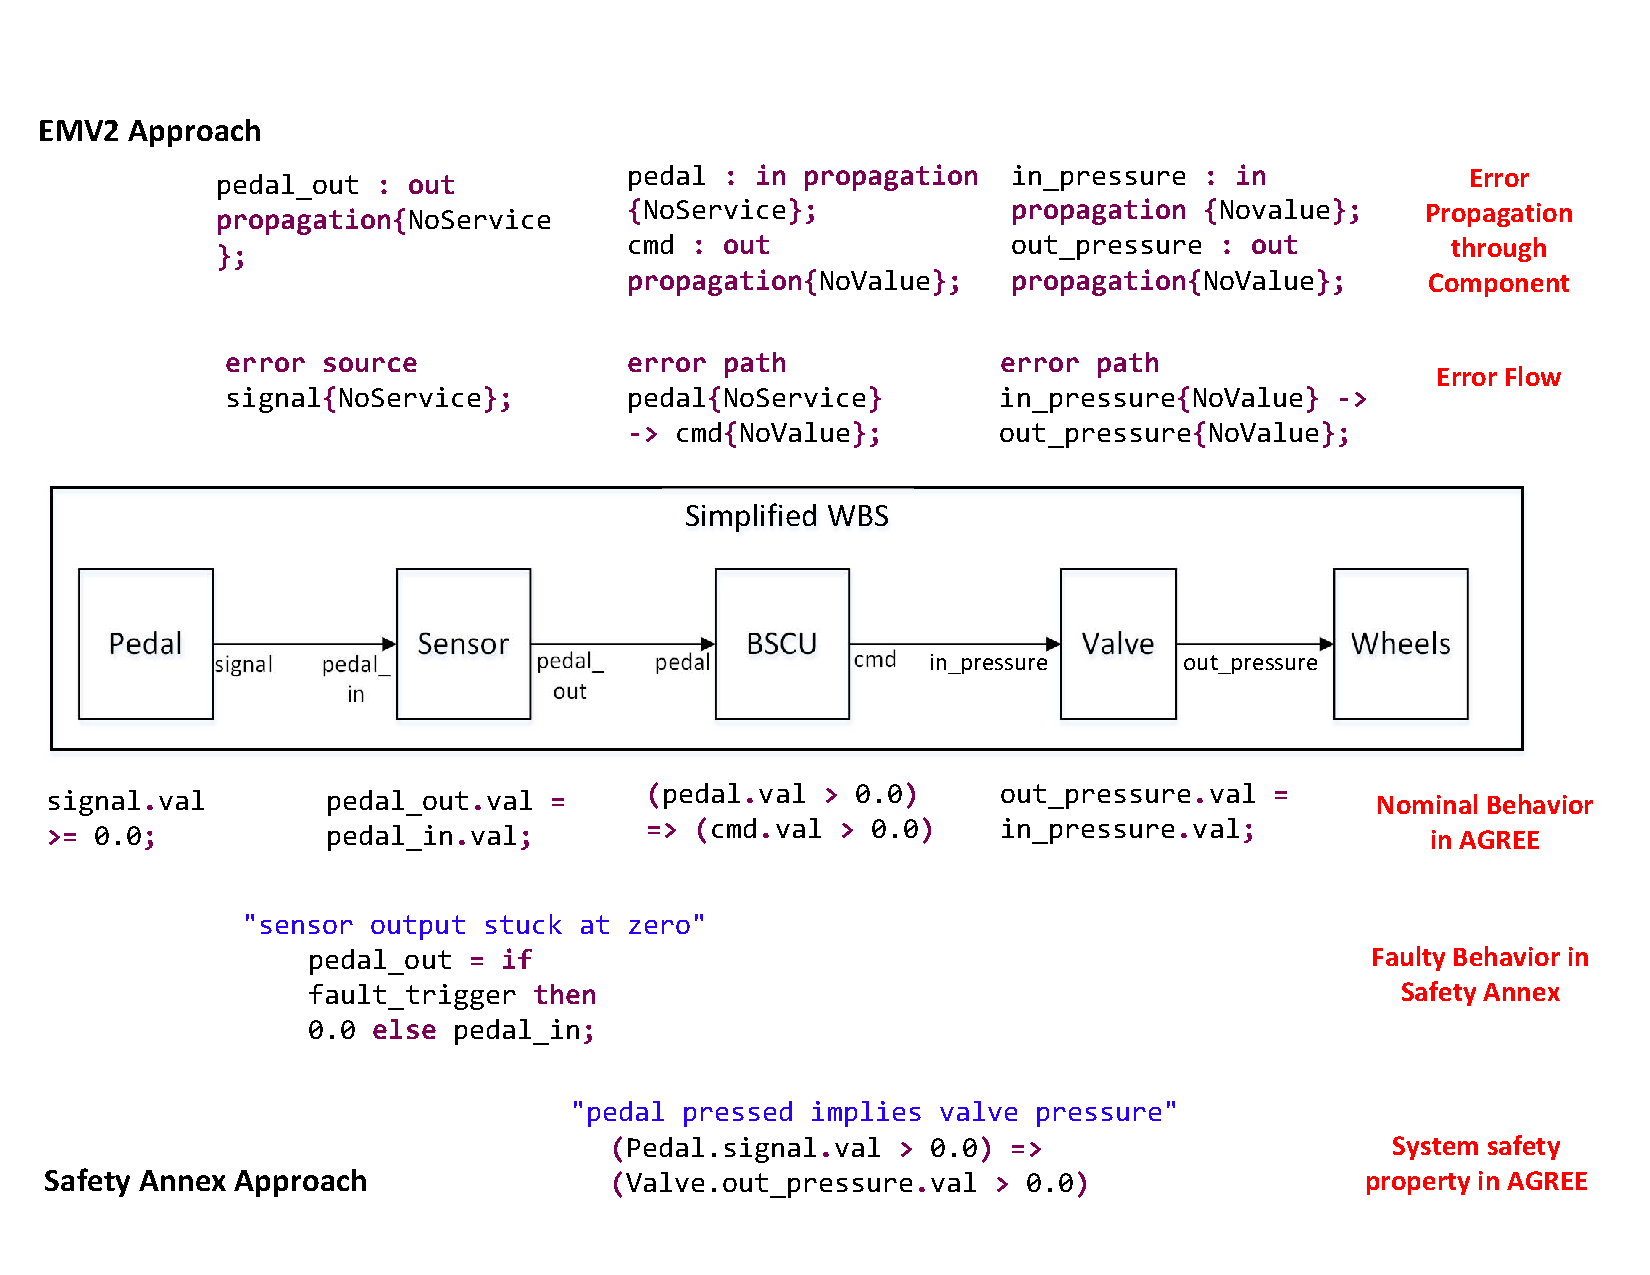
\includegraphics[trim=0 9 0 5,clip,width=\textwidth]{images/Comparison_with_EMV2.pdf}
	%\vspace{-0.3in}
	\caption{Differences between Safety Annex and EMV2}
	\label{fig:comparison_with_EMV2}
	%\vspace{-0.2in}
\end{figure} 

In this simplified WBS system, the physical signal from the Pedal component is detected by the Sensor and the pedal position value is passed to the Braking System Control Unit (BSCU) components.  The BSCU generates a pressure command to the Valve component which applies hydraulic brake pressure to the Wheels. 

In the EMV2 approach (top half of Figure~\ref{fig:comparison_with_EMV2}), the ``NoService'' fault is explicitly propagated through all of the components. These fault types are essentially tokens that do not capture any analyzable behavior. At the system level, analysis tools supporting the EMV2 annex can aggregate the propagation information from different components to compose an overall fault flow diagram or fault tree. 

When a fault is triggered in the Safety Annex (bottom half of Figure~\ref{fig:comparison_with_EMV2}), the output behavior of the Sensor component is modified. In this case the result is a ``stuck at zero'' error. The behavior of the BSCU receives a zero input and proceeds as if the pedal has not been pressed. This will cause the top level system contract to fail: {\em pedal pressed implies brake pressure output is positive}.


\subsection{Explicit Propagation} 
%Faults
Failures in hardware (HW) components can trigger behavioral faults in the system components that depend on them. For example, a CPU %fault
Failure may trigger faulty behavior in the threads bound to that CPU. In addition, a %fault
failure in one HW component may trigger %faults
failure in other HW components located nearby, such as overheating, fire, or explosion
in the containment location. 
The Safety Annex provides the capability to explicitly model the impact of hardware %faults
failures on other faults, behavioral or non behavioral. The explicit propagation to non behavioral faults is similar to that provided in EMV2.

To better model %HW dependent faults 
faults at the system level dependent on HW failures, a fault model element is introduced called a \textit{hardware fault}. Users are not required to specify behavioral effects for the HW faults, nor are data ports necessary on which to apply the fault definition. An example of a model component fault declaration is shown below:
\begin{figure}[h!]
	\vspace{-0.1in}
	\begin{center}
	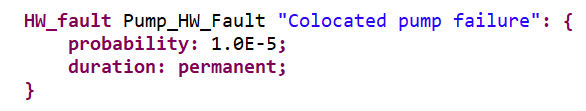
\includegraphics[width=.6\textwidth]{images/hw_fault2.png}
	\end{center}
	\vspace{-0.3in}
	%\caption{Hardware Fault Definition}
	\label{fig:hwFault}
	%\vspace{-0.2in}
	%\vspace{-0.1in}
\end{figure}

Users specify dependencies between the HW component faults and faults that are defined in other components, either HW or SW. The hardware fault then acts as a trigger for dependent faults. This allows a simple propagation from the faulty HW component to the SW components that rely on it, affecting the behavior on the outputs of the affected SW components.

%As an example, we will look yet again at the WBS. 
In the WBS example, assume that both the green and blue hydraulic pumps are located in the same compartment in the aircraft and an explosion in this compartment rendered both pumps inoperable.
%An accident took place and the green (normal) hydraulic pump took the force of an explosion. When the green hydraulic pump exploded, the pump shrapnel flew into the blue pump and it became from then on unoperable. 
The HW fault definition can be modeled first in the green hydraulic pump component as shown in Figure~\ref{fig:hwFault}. The activation of this fault triggers the activation of related faults as seen in the \textit{propagate\_to} statement shown below. % in Figure~\ref{fig:hwFaultProp}. 
Notice that these pumps need not be connected through a data port in order to specify this propagation. %Furthermore, the probability of the HW fault activation can be specified. 

\begin{figure}[h!]
	\vspace{-0.1in}
	\begin{center}
		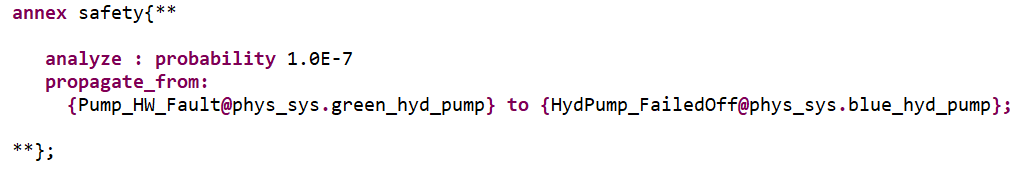
\includegraphics[width=1.0\textwidth]{images/hw_prop_stmt.png}
	\end{center}
	\vspace{-0.3in}
	%\caption{Hardware Fault Propagation Statement}
	\label{fig:hwFaultProp}
	%\vspace{-0.2in}
	%\vspace{-0.1in}
\end{figure}

The fault dependencies are specified in the system implementation where the system configuration that causes the dependencies becomes clear (e.g., binding between SW and HW components, co-location of HW components). 
%This is because fault propagations are typically tied to the way components are connected or bound together; this information may not be available when faults are being specified for individual components. Having fault propagations specified outside of a component’s fault statements also makes it easier to reuse the component in different systems. 



\section{Fault Analysis Statements}
%An annotation in the AADL model determines the fault analysis statement (also referred to in this report as the fault hypothesis). This may specify either a maximum number of faults that can be active at any point in execution:
The fault analysis statement (also referred to as the fault hypothesis) resides in the AADL system implementation that is selected for verification. This may specify either a maximum number of faults that can be active at any point in execution:

\begin{figure}[h!]
	\vspace{-0.1in}
	%\begin{center}
		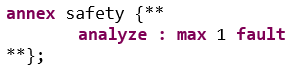
\includegraphics[width=0.4\textwidth]{images/hypothesisMaxN.png}
	%\end{center}
	\vspace{-0.1in}
	%%\caption{Max N Faults Analysis Statement}
	\label{fig:hypothesisMaxN}
\end{figure}
or that the only faults to be considered are those whose probability of simultaneous occurrence is above some probability threshold: 

\begin{figure}[h!]
	\vspace{-0.1in}
	%\begin{center}
		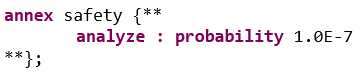
\includegraphics[width=0.5\textwidth]{images/hypothesisProb.png}
	%\end{center}
	\vspace{-0.1in}
	%\caption{Probability Analysis Statement}
	%\label{fig:hypothesisProb}
\end{figure}

Tying back to the fault tree analysis in traditional safety analysis, the former is analogous to restricting the cutsets to a specified maximum number of terms, and the latter is analogous to restricting the cutsets to only those whose probability is above some set value. In the former case, we assert that the sum of the true {\em fault\_\_trigger} variables is at or below some integer threshold.  In the latter, we determine all combinations of faults whose probabilities are above the specified probability threshold, and describe this as a proposition over {\em fault\_\_trigger} variables. 
%
With the introduction of dependent faults, active faults are divided into two categories: independently active (activated by its own triggering event) and dependently active (activated when the faults they depend on become active). The top level fault hypothesis applies to independently active faults. Faulty behaviors augment nominal behaviors whenever their corresponding faults are active (either independently active or dependently active).

\section{Asymmetric Fault Modeling}
\label{sec:byzantine}
A \textit{asymmetric} or \textit{Byzantine} fault is a fault that presents different symptoms to different observers~\cite{Driscoll-Byzantine-Fault}. In our modeling environment, asymmetric faults may be associated with a component that has a one-to-many ($1-n$) output to multiple ($n$) other components. In this configuration, a \textit{symmetric} fault will result in all destination components seeing the same faulty behavior from the source component. To capture the behavior of asymmetric faults (``different symptoms to different observers''), it was necessary to extend our fault modeling mechanism in AADL. A thorough description of the asymmetric modeling capability of the Safety Annex is shown in Chapter~\ref{chap:caseStudies} using a process ID example.

\subsection{Implementation of Asymmetric Faults}
To illustrate our implementation of asymmetric faults, assume a source component A has a 1-n output connected to four destination components (B-E) as shown in Figure~\ref{fig:commNodes} under ``Nominal System.'' If a symmetric fault was present on this output, all four connected components would see the same faulty behavior. An asymmetric fault should be able to present arbitrarily different values to the connected components. 

To this end, ``communication nodes'' are inserted on each connection from component A to components B, C, D, and E (shown in Figure~\ref{fig:commNodes} under ``Fault Model Architecture.'' From the users perspective, the asymmetric fault definition is associated with component A's output and the architecture of the model is unchanged from the nominal model architecture. Behind the scenes, these communication nodes are created to facilitate potentially different fault activations on each of these connections. The fault definition used on the output of component A will be inserted into each of these communication nodes as shown by the red circles at the communication node output in Figure~\ref{fig:commNodes}.
\begin{figure}[!htb]
        \center{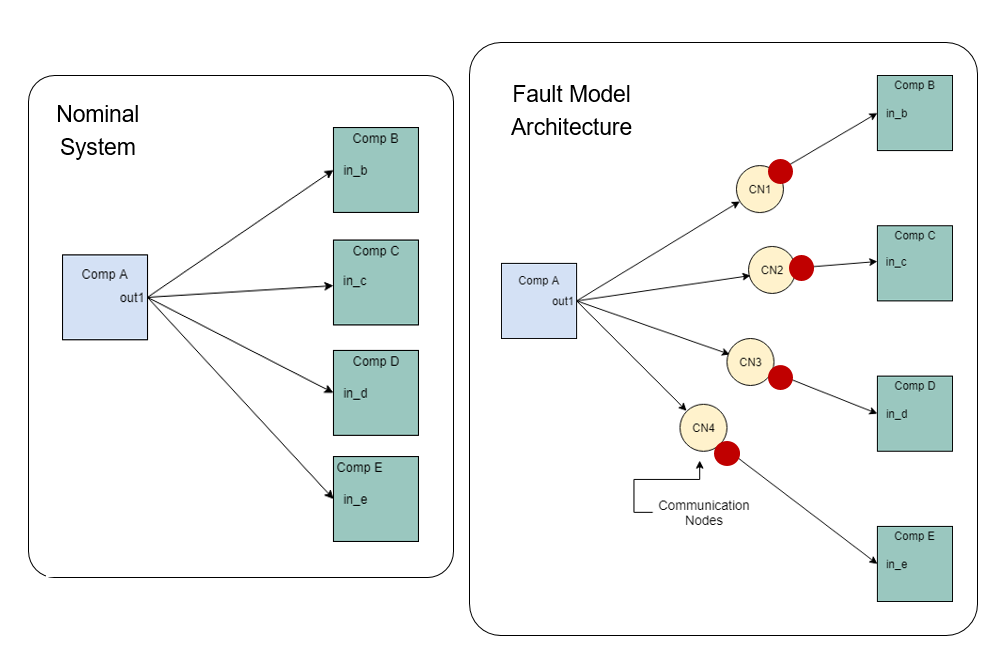
\includegraphics[width=\textwidth] {images/commNodes.png}}
        \caption{\label{fig:commNodes} Communication Nodes in Asymmetric Fault Implementation}
\end{figure}

\begin{figure}[!htb]
        \center{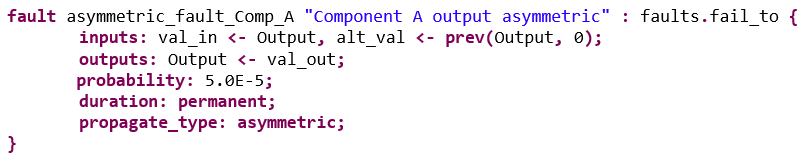
\includegraphics[width=\textwidth] {images/asymFaultDef.png}}
        \caption{\label{fig:asymFaultDef} Asymmetric Fault Definition in the Safety Annex}
\end{figure}

An asymmetric fault is defined for Component A as in Figure~\ref{fig:asymFaultDef}. This fault defines an asymmetric failure on Component A that when active, is stuck at a previous value (\textit{prev(Output, 0)}). This can be interpreted as the following: some connected components may only see the previous value of Comp A output and others may see the correct (current) value when the fault is active. This fault definition is injected into the communication nodes and which of the connected components see an incorrect value is completely nondeterministic. Any number of the communication node faults (0…all) may be active upon activation of the main asymmetric fault.

%\subsection{Referencing Fault Activation Status}
%To fully implement the agreement protocol, it must be possible to describe whether or not a subcomponent is failed by specifying if any faults defined for the subcomponents is activated. In the Safety Annex, this is made possible through the use of a \textit{fault activation} statement. Users can declare boolean \textit{eq} variables in the AGREE annex of the AADL system where the AGREE verification applies to that system's implementation. %in AGREE and in the implementations Safety Annex,  Users can then assign the activation status of specific faults to those \textit{eq} variables in Safety Annex of the AADL system implementation (the same place where the fault analysis statement resides).
%assigns this boolean \textit{eq} statement to a fault specific to a subcomponent.  This assignment links each specified AGREE boolean variable with the activation status of the specified fault activation literal. The AGREE boolean variable is true when and only when the fault is active. This additional feature of the Safety Annex allows users to state contracts of the form: if \texttt{sensor\_failed} then \texttt{do\_something}.

 









